\section{Geometric primitives}

\subsection{Lines and rays}

Types of lines:
\begin{enumerate}
	\item Infinite line in both directions.
	\item Line segment: finite line between two points.
	\item Ray Some origin and infinite extension in some direction. In computer graphics we often make use of a finite ray however.
\end{enumerate}

\subsection{Spheres and circles}

Some important functions with regards to spheres and circles.

\begin{itemize}
	\item Implicit definition of 2D circle: $(x-c_x)^2 + (y-c_y)^2=r^2$
	\item Implicit definition of 3D sphere: $(x-c_x)^2 + (y-c_y)^2+ (z-c_z)^2=r^2$
	\item Common formulas:
	\begin{align*}
		D &= 2r &(\text{diameter}) \\
		C &= 2\pi{}r = \pi{}D &(\text{circumference}) \\
		A &= \pi{}r^2 &(\text{area of circle}) \\
		S &= 4\pi{}r^2 &(\text{surface area of sphere}) \\
		V &= \frac{4}{3}\pi{}r^3 &(\text{volume of sphere})
	\end{align*}
\end{itemize}

\subsection{Bounding boxes}

Types of bounding boxes:
\begin{enumerate}
	\item AABB: the box is aligned to the world's axes.
	\begin{itemize}
		\item All points are defined by:
		\begin{align*}
			x_{min} &\leq x \leq x_{max} \\ 
			y_{min} &\leq y \leq y_{max} \\
			z_{min} &\leq z \leq z_{max}
		\end{align*}
		\item $p_{min}=\begin{bmatrix}
			x_{min} & y_{min} & z_{min}
		\end{bmatrix}$
		\item $p_{max}=\begin{bmatrix}
			x_{max} & y_{max} & z_{max}
		\end{bmatrix}$
		\item $center= (p_{min} + p_{max}) / 2$
		\item $size = p_{max} - p_{min}$
		\item $radius = size / 2$
	\end{itemize}
	\item OBB: the box is aligned in object space.
	\item Spheres can also be used as bounding box (uh sphere). They are easy to use for intersection, but often poorly wrap around objects.
\end{enumerate}

\subsection{Planes}

\begin{itemize}
	\item Implicit definition of a plane: $\textbf{p} \cdot \hat{\textbf{n}}=d$. Where $\textbf{n}$ is the vector perpendicular to the plane and $d$ the distance from the origin.
	\item The plane normal ($\hat{\textbf{n}}$) can be calculated for any three noncollinear points with the following formulas:
	\begin{enumerate}
		\item $\textbf{e}_3 = \textbf{p}_2 - \textbf{p}_1$,
		\item $\textbf{e}_1 = \textbf{p}_3 - \textbf{p}_2$,
		\item $\hat{\textbf{n}}=\frac{\textbf{e}_3 \times \textbf{e}_1}{\| \textbf{e}_3 \times \textbf{e}_1 \|}$.
		\item $d=\hat{\textbf{n}} \cdot \textbf{p}_1$
	\end{enumerate}
	\item Distance of some point, $\textbf{q}$, to the plane can be computed with the formula: $distance = \textbf{q} \cdot \hat{\textbf{n}} - d$.
	\item See exercise 5 of chapter 9 for an interesting algorithm to find the best fit plane for a set of points.
\end{itemize}

\subsection{Triangles}

\subsubsection{Notation}

In a left-handed system the vertices of triangles are defined clockwise, while in right-handed system the vertices are defined counter-clockwise.

\begin{figure}[H]
\centering
    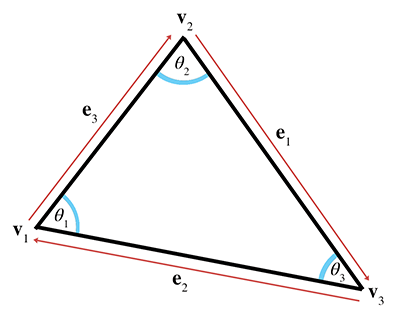
\includegraphics{09_triangle_notation}
\caption{Triangle notation}
\label{fig:triangle-notation}
\end{figure}

Formulas for all edges and lengths:

\begin{align*}
\textbf{e}_1 &= \textbf{v}_3 - \textbf{v}_2, & \textbf{e}_2 &= \textbf{v}_1 - \textbf{v}_3, & \textbf{e}_3 &= \textbf{v}_2 - \textbf{v}_1, \\
l_1& = \|\textbf{e}_1\|, & l_2 &= \|\textbf{e}_2\|, & l_3 &= \|\textbf{e}_3\|, \\
\end{align*}

The perimeter is defined by the sum of lengths: $p = l_1 + l_2 + l_3$.

Also, remember the sine and cosine laws from section \ref{sin_cos_laws}.

\subsubsection{Area}

The triangle area can be calculated with $\frac{\text{base}\cdot{}\text{height}}{2}$. A second approach is using the cross product: 

$$A=\frac{\| \textbf{e}_1 \times \textbf{e}_2 \|}{2}$$

\noindent{} Personally, I like this approach best. It works for 3D and 2D.

\subsubsection{Barycentric coordinates}

A barycentric coordinate is the weighted average of the three vertices of a triangle. $(b_1, b_2, b_3) \equiv (b_1\textbf{v}_1+b_2\textbf{v}_2+b_3\textbf{v}_3)$. The requirement is that $b_1+b_2+b_3=1$.

\begin{figure}[H]
\centering
    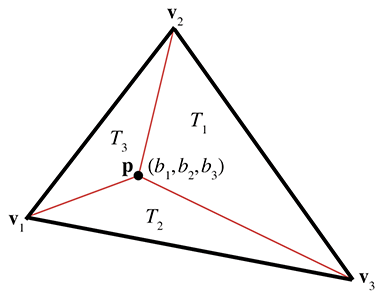
\includegraphics{09_barycentric_coordinates}
\caption{Barycentric coordinates}
\label{fig:barycentric-coordinates}
\end{figure}

Refer the book and the \path{exercise04.cpp} in \path{chapter09} for algorithms to compute barycentric coordinates.

\subsubsection{Center of gravity}

\begin{figure}[H]
\centering
    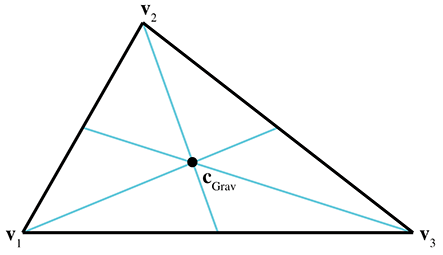
\includegraphics{09_center_of_gravity}
\caption{Center of gravity}
\label{fig:center-of-gravity}
\end{figure}

The center of gravity can be computed as follows:

$$\textbf{c}_{\text{Gravity}}= \frac{\textbf{v}_1+\textbf{v}_2+\textbf{v}_3}{3}$$

\noindent Barycentric notation: 

$$\left( \frac{1}{3}, \frac{1}{3}, \frac{1}{3} \right)$$

\subsubsection{Incenter}

\begin{figure}[H]
\centering
    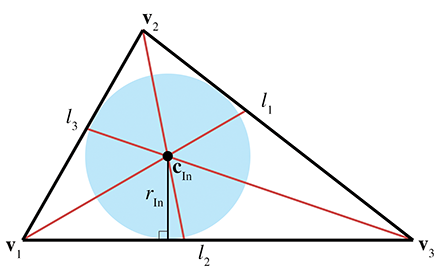
\includegraphics{09_incenter}
\caption{Incenter}
\label{fig:incenter}
\end{figure}

The incenter is computed by:

$$\textbf{c}_{\text{In}} = \frac{l_1\textbf{v}_1 + l_2\textbf{v}_2 + l_3\textbf{v}_3}{p}$$

\noindent Barycentric notation:

$$\left(\frac{l_1}{p}, \frac{l_2}{p}, \frac{l_3}{p}\right)$$

\noindent Radius of incenter:

$$r_{\text{In}} = \frac{A}{p}$$

\subsubsection{Circumcenter}

\begin{figure}[H]
\centering
    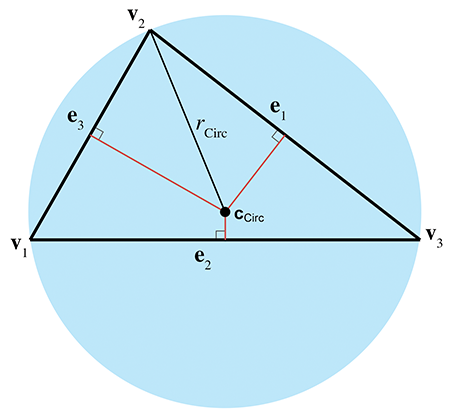
\includegraphics{09_circumcenter}
\caption{Circumcenter}
\label{fig:circumcenter}
\end{figure}

The circumcenter is the point the is equidistant from all vertices. It solves the problem of finding a circle that passes through three points. The computation is a bit length, so just refer the book whenever you need this.

\subsection{Polygons}

Polygons are quite hard to define, but basically it are shapes made up of vertices and edges. Some important terms to know about:

\begin{itemize}
	\item \textit{Simple} polygon: a polygon without any holes.
	\item \textit{Complex} polygon: a polygon that may have holes.
	
\begin{figure}[H]
\centering
    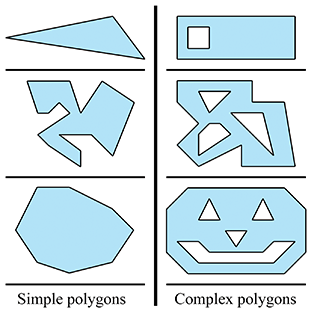
\includegraphics{09_simple_complex}
\caption{Simple and complex polygons}
\label{fig:simple-complex-polygons}
\end{figure}

	\item \textit{Convex} polygon: a polygon without dents, all edges between all vertices are contained in the polygon.
	\item \textit{Concave} polygon: a polygon with some dent, at least one edge between any pair of vertices is outside the polygon.
	
\begin{figure}[H]
\centering
    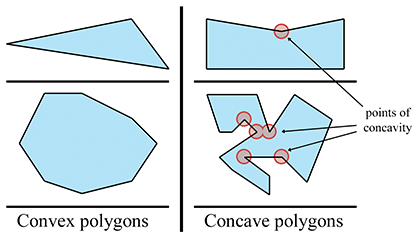
\includegraphics{09_convex_concave}
\caption{Convex and concave polygons}
\label{fig:convex-concave-polygons}
\end{figure}	
	
	\item Polygons can be divided into triangles. For complex polygons this is quite tricky, but for any convex it is quite easy. It can be done by a method called \textit{fanning}, which basically adds extra edges to subdivide the polygon into triangles.
\begin{figure}[H]
\centering
    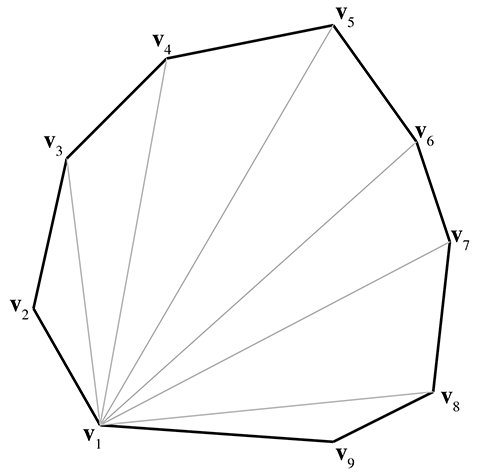
\includegraphics{09_fanning}
\caption{Fanning of convex polygon}
\label{fig:convex-fanning}
\end{figure}

\end{itemize}
